%
% problemstellung.tex 
%
% 
%
% !TEX root = ../../buch.tex
% !TEX encoding = UTF-8
%

\section{Aufgabenstellung\label{antennen:problemstellung}}
\rhead{Aufgabenstellung}
 Es soll eine Antennenform designed werden, welche in einem Gerät mit der Form 
 eines Prismas mit Deckfläche eines gleichseitigen Dreiecks. Dies bedeutet, dass 
 die Form das Mass eines gleichseitigen Dreiecks nicht überschreiten darf.
 
\subsection{Geometrie\label{antennen:Geom}}
\rhead{Geometrie}
Das Ziel ist nun, den Wirkungsgrad durch Formoptimierung zu erhöhen. Somit soll eine optimale Form
gefunden werden, welche vorherige Einschränkungen einhält.
Die Faktoren $k\textsubscript{1}$ und $k\textsubscript{2}$ sind Konstanten, 
was bedeutet, dass für eine Erhöhung des Wirkungsgrads \eqref{antennen:Wirkungsgradeingesetzt} nur die Länge 
$l$ und die Fläche $A$ relevant und veränderbar sind. In einem nächsten Schritt wird das Verhältnis
\begin{equation}
	\frac{l}{A^2} \rightarrow \frac{l}{A}
	\label{antennen:Verhältnis}
\end{equation}
erhöht. 
Die grösste Fläche ist auch gerade die grösste Fläche im Quadrat. Somit können wir diesen Ausdruck 
für den weiteren Verlauf vereinfachen. Diese vereinfachte Formel kann nun auf eine implizite 
Funktion angewendet werden. Die Funktion gibt dann Auskunft über die aufgespannte Fläche und 
dem Umfang. Somit kann das Verhältnis \eqref{antennen:Verhältnis} gezielt optimiert werden. 

Eine erste, nicht mathematische, Idee besteht darin, die Ecken abzuflachen. Da sonst in den Ecken
eines Dreiecks viel zusätzliche Länge und nur wenig Fläche gewonnen wird. Dies ist in der Abbildung
\ref{antennen:tikabgeflacht} zu sehen. 

Eine weitere Idee wäre es die Ecken wie in der Abbildung \ref{antennen:tikabgerundet} abzuflachen. Bei
beiden Ideen muss noch bestimmt werden, wo genau die Anpassung der Eckstücke gemacht werden muss um 
das Verhältnis \eqref{antennen:Verhältnis} zu optimieren. Dies ist in den Abbildungen 
\ref{antennen:tikabgeflacht_kleiner} und \ref{antennen:tikabgerundet_kleiner} veranschaulicht.

\begin{figure}
	\centering
	\begin{minipage}[t]{0.45\textwidth}
		\centering
		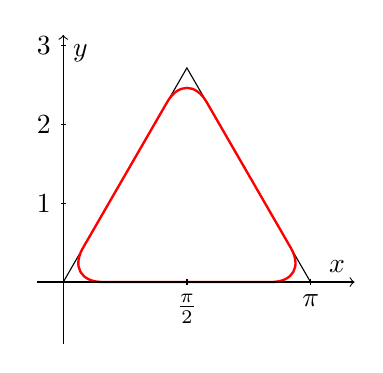
\begin{tikzpicture}

			\def\sidelength{3.14}
			
			\pgfmathsetmacro{\triangleheight}{sqrt(3)/2*\sidelength}

			\draw[fill=white] (0,0) -- (\sidelength,0) -- (0.5*\sidelength, \triangleheight) -- cycle;
			
			\draw[red, line width=0.3mm, rounded corners=0.5cm] (0,0) -- (\sidelength,0) -- (0.5*\sidelength, \triangleheight) -- cycle;
			
			\draw[->] (-0.33,0) -- (3.7,0) node[above left] {$x$};
			\draw[->] (0,-0.785) -- (0,3.14) node[below right] {$y$};
			
			\foreach \x\xlabel in {1.5708/$\frac{\pi}{2}$, 3.14159/$\pi$}
			\draw (\x,1pt) -- (\x,-1pt) node[below] {\xlabel};
			\foreach \y in {1, 2, 3}
			\draw (1pt,\y) -- (-1pt,\y) node[left] {\y};
		\end{tikzpicture}
		\caption{Antenne mit abgerundeten Ecken}
		\label{antennen:tikabgerundet}
	\end{minipage}
	\hfill
	\begin{minipage}[t]{0.45\textwidth}
		\centering
		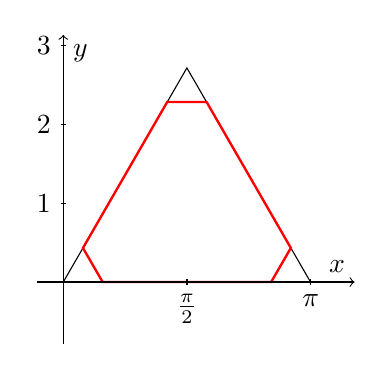
\begin{tikzpicture}
			\def\sidelength{3.14}
			
			\pgfmathsetmacro{\triangleheight}{sqrt(3)/2*\sidelength}

			\draw[fill=white] (0,0) -- (\sidelength,0) -- (0.5*\sidelength, \triangleheight) -- cycle;
			
			\draw[red, line width=0.3mm] 
			(0.5,0) -- (0.25,1.73/2*0.5) -- (0.5*\sidelength-0.25, \triangleheight-1.73/2*0.5) -- 
			(0.5*\sidelength+0.25, \triangleheight-1.73/2*0.5) -- (\sidelength-0.25,1.73/2*0.5) -- (\sidelength-0.5,0) -- cycle;
			
			\draw[->] (-0.33,0) -- (3.7,0) node[above left] {$x$};
			\draw[->] (0,-0.785) -- (0,3.14) node[below right] {$y$};
			
			\foreach \x\xlabel in {1.5708/$\frac{\pi}{2}$, 3.14159/$\pi$}
			\draw (\x,1pt) -- (\x,-1pt) node[below] {\xlabel};
			\foreach \y in {1, 2, 3}
			\draw (1pt,\y) -- (-1pt,\y) node[left] {\y};
		\end{tikzpicture}
		\caption{Antennenform mit abgeflachten Ecken}
		\label{antennen:tikabgeflacht}
	\end{minipage}


\end{figure}

\begin{figure}
	\centering
	\begin{minipage}[t]{0.45\textwidth}
		\centering
		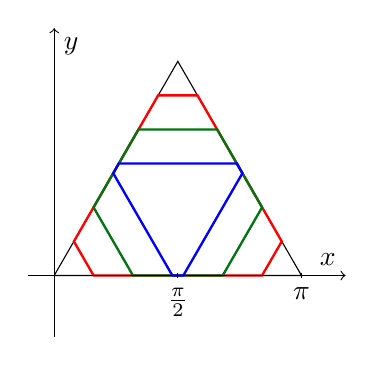
\begin{tikzpicture}
			\definecolor{clrGreen}{RGB}{0, 117, 18}

			\def\sidelength{3.14}
			
			\pgfmathsetmacro{\triangleheight}{sqrt(3)/2*\sidelength}

			\draw[fill=white] (0,0) -- (\sidelength,0) -- (0.5*\sidelength, \triangleheight) -- cycle;
			
			\draw[red, line width=0.3mm,] (0.5,0) -- (0.25,1.73 /2*0.5) -- (0.5*\sidelength-0.25, \triangleheight-1.73/2*0.5) -- (0.5*\sidelength+0.25, \triangleheight-1.73/2*0.5)--(\sidelength-0.25,1.73/2*0.5) -- (\sidelength-0.5,0) -- cycle;
			
			\draw[clrGreen, line width=0.3mm,] (1,0) -- (0.5,1.73 /2*1) -- (0.5*\sidelength-0.5, \triangleheight-1.73/2*1) -- (0.5*\sidelength+0.5, \triangleheight-1.73/2*1)--(\sidelength-0.5,1.73/2*1) -- (\sidelength-1,0) -- cycle;
			
			\draw[blue, line width=0.3mm,] (1.5,0) -- (0.75,1.73 /2*1.5) -- (0.5*\sidelength-0.75, \triangleheight-1.73/2*1.5) -- (0.5*\sidelength+0.75, \triangleheight-1.73/2*1.5)--(\sidelength-0.75,1.73/2*1.5) -- (\sidelength-1.5,0) -- cycle;
			
			\draw[->] (-0.33,0) -- (3.7,0) node[above left] {$x$};
			\draw[->] (0,-0.785) -- (0,3.14) node[below right] {$y$};
			
			\foreach \x/\xlabel in {1.5708/$\frac{\pi}{2}$, 3.14159/$\pi$}
			\draw (\x,1pt) -- (\x,-1pt) node[below] {\xlabel};
		\end{tikzpicture}
		\caption{Antennenform mit variablen abgeflachten Ecken}
		\label{antennen:tikabgeflacht_kleiner}
	\end{minipage}
	\hfill
	\begin{minipage}[t]{0.45\textwidth}
		\centering
		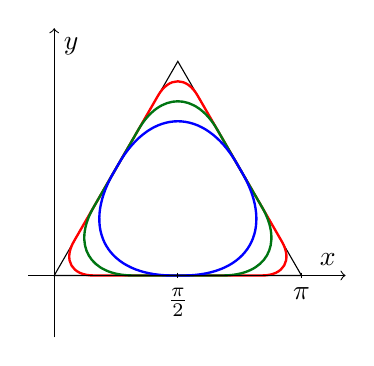
\begin{tikzpicture}
			\definecolor{clrGreen}{RGB}{0, 117, 18}

			\def\sidelength{3.14}
			
			\pgfmathsetmacro{\triangleheight}{sqrt(3)/2*\sidelength}

			\draw[fill=white] (0,0) -- (\sidelength,0) -- (0.5*\sidelength, \triangleheight) -- cycle;
			
			\draw[red, line width=0.3mm, rounded corners=0.5cm] (0,0) -- (\sidelength,0) -- (0.5*\sidelength, \triangleheight) -- cycle;
			
			\draw[clrGreen, line width=0.3mm, rounded corners=1cm] (0,0) -- (\sidelength,0) -- (0.5*\sidelength, \triangleheight) -- cycle;
			
			\draw[blue, line width=0.3mm, rounded corners=1.5cm] (0,0) -- (\sidelength,0) -- (0.5*\sidelength, \triangleheight) -- cycle;
			
			\draw[->] (-0.33,0) -- (3.7,0) node[above left] {$x$};
			\draw[->] (0,-0.785) -- (0,3.14) node[below right] {$y$};
			
			\foreach \x/\xlabel in {1.5708/$\frac{\pi}{2}$, 3.14159/$\pi$}
			\draw (\x,1pt) -- (\x,-1pt) node[below] {\xlabel};
		\end{tikzpicture}
		\caption{Antennenform mit variablen abgerundeten Ecken}
		\label{antennen:tikabgerundet_kleiner}
	\end{minipage}%
\end{figure}
\FloatBarrier
Eine Eigenschaft, die das Problem vereinfacht, ist die Symmetrie des Dreiecks. 
Das Gesamtproblem kann vereinfacht werden indem nur eine Ecke betrachtet wird. 
Wie in den Abbildungen \ref{antennen:tiksymmetrie} und \ref{antennen:Ecke} dargestellt, sind die drei Eckfunktionen äquivalent. Die drei 
gestrichelten Geraden spannen ein weiteres gleichseitiges Dreieck auf, das 
jedoch vernachlässigt werden kann, da dieses für alle gesuchten Funktionen $f(x,y)$ 
gleich bleibt. Somit ist das implizite Problem $f(x,y)$ zur expliziten Funktion $f(x)$ 
geworden, die wesentlich leichter zu optimieren ist.
\begin{figure}
	\centering
	\begin{minipage}[b]{0.45\textwidth}
		\centering
		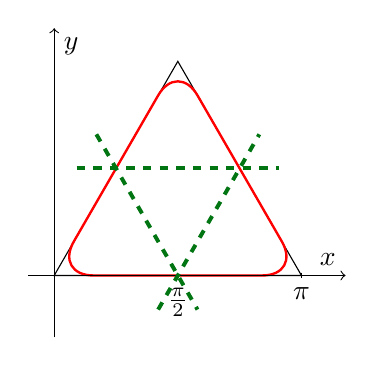
\begin{tikzpicture}
			\definecolor{clrGreen}{RGB}{0, 117, 18}

			\def\sidelength{3.14}
			
			\pgfmathsetmacro{\triangleheight}{sqrt(3)/2*\sidelength}

			\draw[fill=white] (0,0) -- (\sidelength,0) -- (0.5*\sidelength, \triangleheight) -- cycle;
			
			\draw[red, line width=0.3mm, rounded corners=0.5cm] (0,0) -- (\sidelength,0) -- (0.5*\sidelength, \triangleheight) -- cycle;
			
			\draw[->] (-0.33,0) -- (3.7,0) node[above left] {$x$};
			\draw[->] (0,-0.785) -- (0,3.14) node[below right] {$y$};
			
			\foreach \x/\xlabel in {1.5708/$\frac{\pi}{2}$, 3.14159/$\pi$}
			\draw (\x,1pt) -- (\x,-1pt) node[below] {\xlabel};
			
			\draw[clrGreen, dashed, line width=0.5mm] (3.14156/4-0.5, \triangleheight/2) -- (0.75*\sidelength+0.5, \triangleheight/2);
			\draw[clrGreen, dashed, line width=0.5mm] (3.14156/4-0.25, \triangleheight/2+0.433) -- (0.5*\sidelength+0.25, 0-0.433);
			\draw[clrGreen, dashed, line width=0.5mm] (0.5*\sidelength-0.25, 0-0.433) -- (0.75*\sidelength+0.25, \triangleheight/2+0.433);
		\end{tikzpicture}
		\caption{Symmetrie einer Antenne}
		\label{antennen:tiksymmetrie}
	\end{minipage}%
	\hfill
	\begin{minipage}[b]{0.45\textwidth}
		\centering
		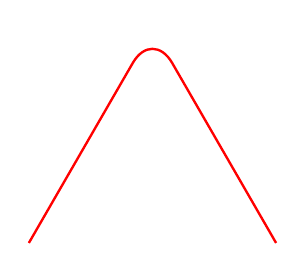
\begin{tikzpicture}

			\def\sidelength{3.14}

			\pgfmathsetmacro{\triangleheight}{sqrt(3)/2*\sidelength}
			
			\draw[red, line width=0.3mm, rounded corners=0.5cm] (0,0) -- (0.5*\sidelength, \triangleheight) -- (\sidelength,0);
		\end{tikzpicture}
		\caption{Eine Ecke der Antenne}
		\label{antennen:Ecke}
	\end{minipage}
\end{figure}







